% !TeX root = proyecto.tex

%=========================================================
\chapter{Modelo del Negocio}	
\label{cap:reqSist}

\cdtInstrucciones{Introduzca el capítulo describiendo el contenido del mismo, su organización y propósito.}

%----------------------------------------------------------
\section{Actores del sistema}

	\cdtInstrucciones{En esta sección describa a los actores del sistema.}
	
	%---------------------------------------------------------
	\begin{Usuario}{\hypertarget{A.NombreDelUsuario}{\subsection{Nombre del usuario}}}{
			Descripción del usuario: su puesto
		}
		\item[Responsabilidades:] \cdtEmpty
		\begin{itemize}
			\item Listar todas las responsabilidades y actividades dentro de la empresa.
			\item ...
		\end{itemize}
		
		\item[Perfil:] \cdtEmpty
		\begin{itemize}
			\item Describa el perfil del puesto: cursos, experiencia,habilidades blandas, escolaridad, certificaciones, etc.
			\item ...
		\end{itemize}
		\item[Procesos en los que participa:] \cdtEmpty
		\begin{itemize}
			\item Liste los procesos en los que participa.
			\item PC-V01 Aprobar las ordenes de compra al mayoreo.
			\item ...
		\end{itemize}
		\item[Área:] Indique el nombre del área a la que pertenece dentro de la organización
		\item[Cantidad aproximada:] Cantidad aproximada de personas que participan con este rol en el negocio.
		\item[Horario actividad:] En qué horario se espera que utilice el sistema. 
	\end{Usuario}
	
%---------------------------------------------------------
\section{Términos del Negocio}
\label{sec:terminosDeNegocio}

\cdtInstrucciones{En esta sección describa todos los términos del negocio que aparecen en la especificación del sistema.}
	
\begin{description}
	% Ejemplo de un término literal.
	\item[\hypertarget{tAutomovil}{Automóvil:}] ({\em es un tipo de \hyperlink{tVehiculo}{Vehículo}}) De cuatro ruedas con capacidad de 5 a 9 personas. 
	% Ejemplo de un término de entidad
	\item[\hypertarget{tCliente}{Cliente:}] Se refiere a todas las personas físicas y morales que \hyperlink{tRenta}{rentan} o han rentado un \hyperlink{tVehiculo}{vehículo}.
	
	\item[\hypertarget{tDirector}{Director:}] ({\em es un tipo de \hyperlink{tEmpleado}{Empleado}}) Es el empleado que tiene mayor rango de todos y no tiene superior, a diferencia de los demás.	
	\item[\hypertarget{tEmpleado}{Empleado:}] Se refiere a cualquier persona que labore en la empresa.
	
	\item[\hypertarget{tChecador}{Checador:}] ({\em Reloj asociado al atributo:} Hora de entrada y salida de un \hyperlink{tEmpleado}{empleado}. {\em Frecuencia de lectura:} Una vez al día para la entrada y otra para la salida durante los días laborales.
	
	\item[\hypertarget{tMotocicleta}{Motocicleta:}] ({\em es un tipo de {tVehiculo}{Vehículo}}) De dos ruedas con capacidad para una personas. 

	\item[\hypertarget{tRenta}{Renta:}] Se refiere al servicio que ofrece la empresa para prestar \hyperlink{tVehiculo}{vehículos} a los \hyperlink{tCliente}{clientes} por un tiempo definido.
	
	\item[\hypertarget{tVehiculo}{Vehiculo:}] Se refiere a los automóviles y motocicletas que la empresa usa para dar el servicio de renta a los \hyperlink{tCliente}{clientes}.
	
%	\brTermSensor{tVelocimetro}{Velocímetro:}{Velocidad de un Vehículo.}{Kilometros/hora.}{Constantemente siempre que el \cdtRef{tVehiculo}{vehículo} esté encendido.}
\end{description}

%----------------------------------------------------------
\section{Modelo del dominio del problema}
\label{sec:hechosDeNegocio}

\cdtInstrucciones{En esta sección describa todas las entidades del negocio y sus relaciones.}

	El modelo del dominio del problema se muestra en la figura~\ref{fig:modeloDeDominio}, a continuación se describen cada una de las entidades y sus relaciones.
	
\begin{figure}[htpb!]
	\begin{center}
		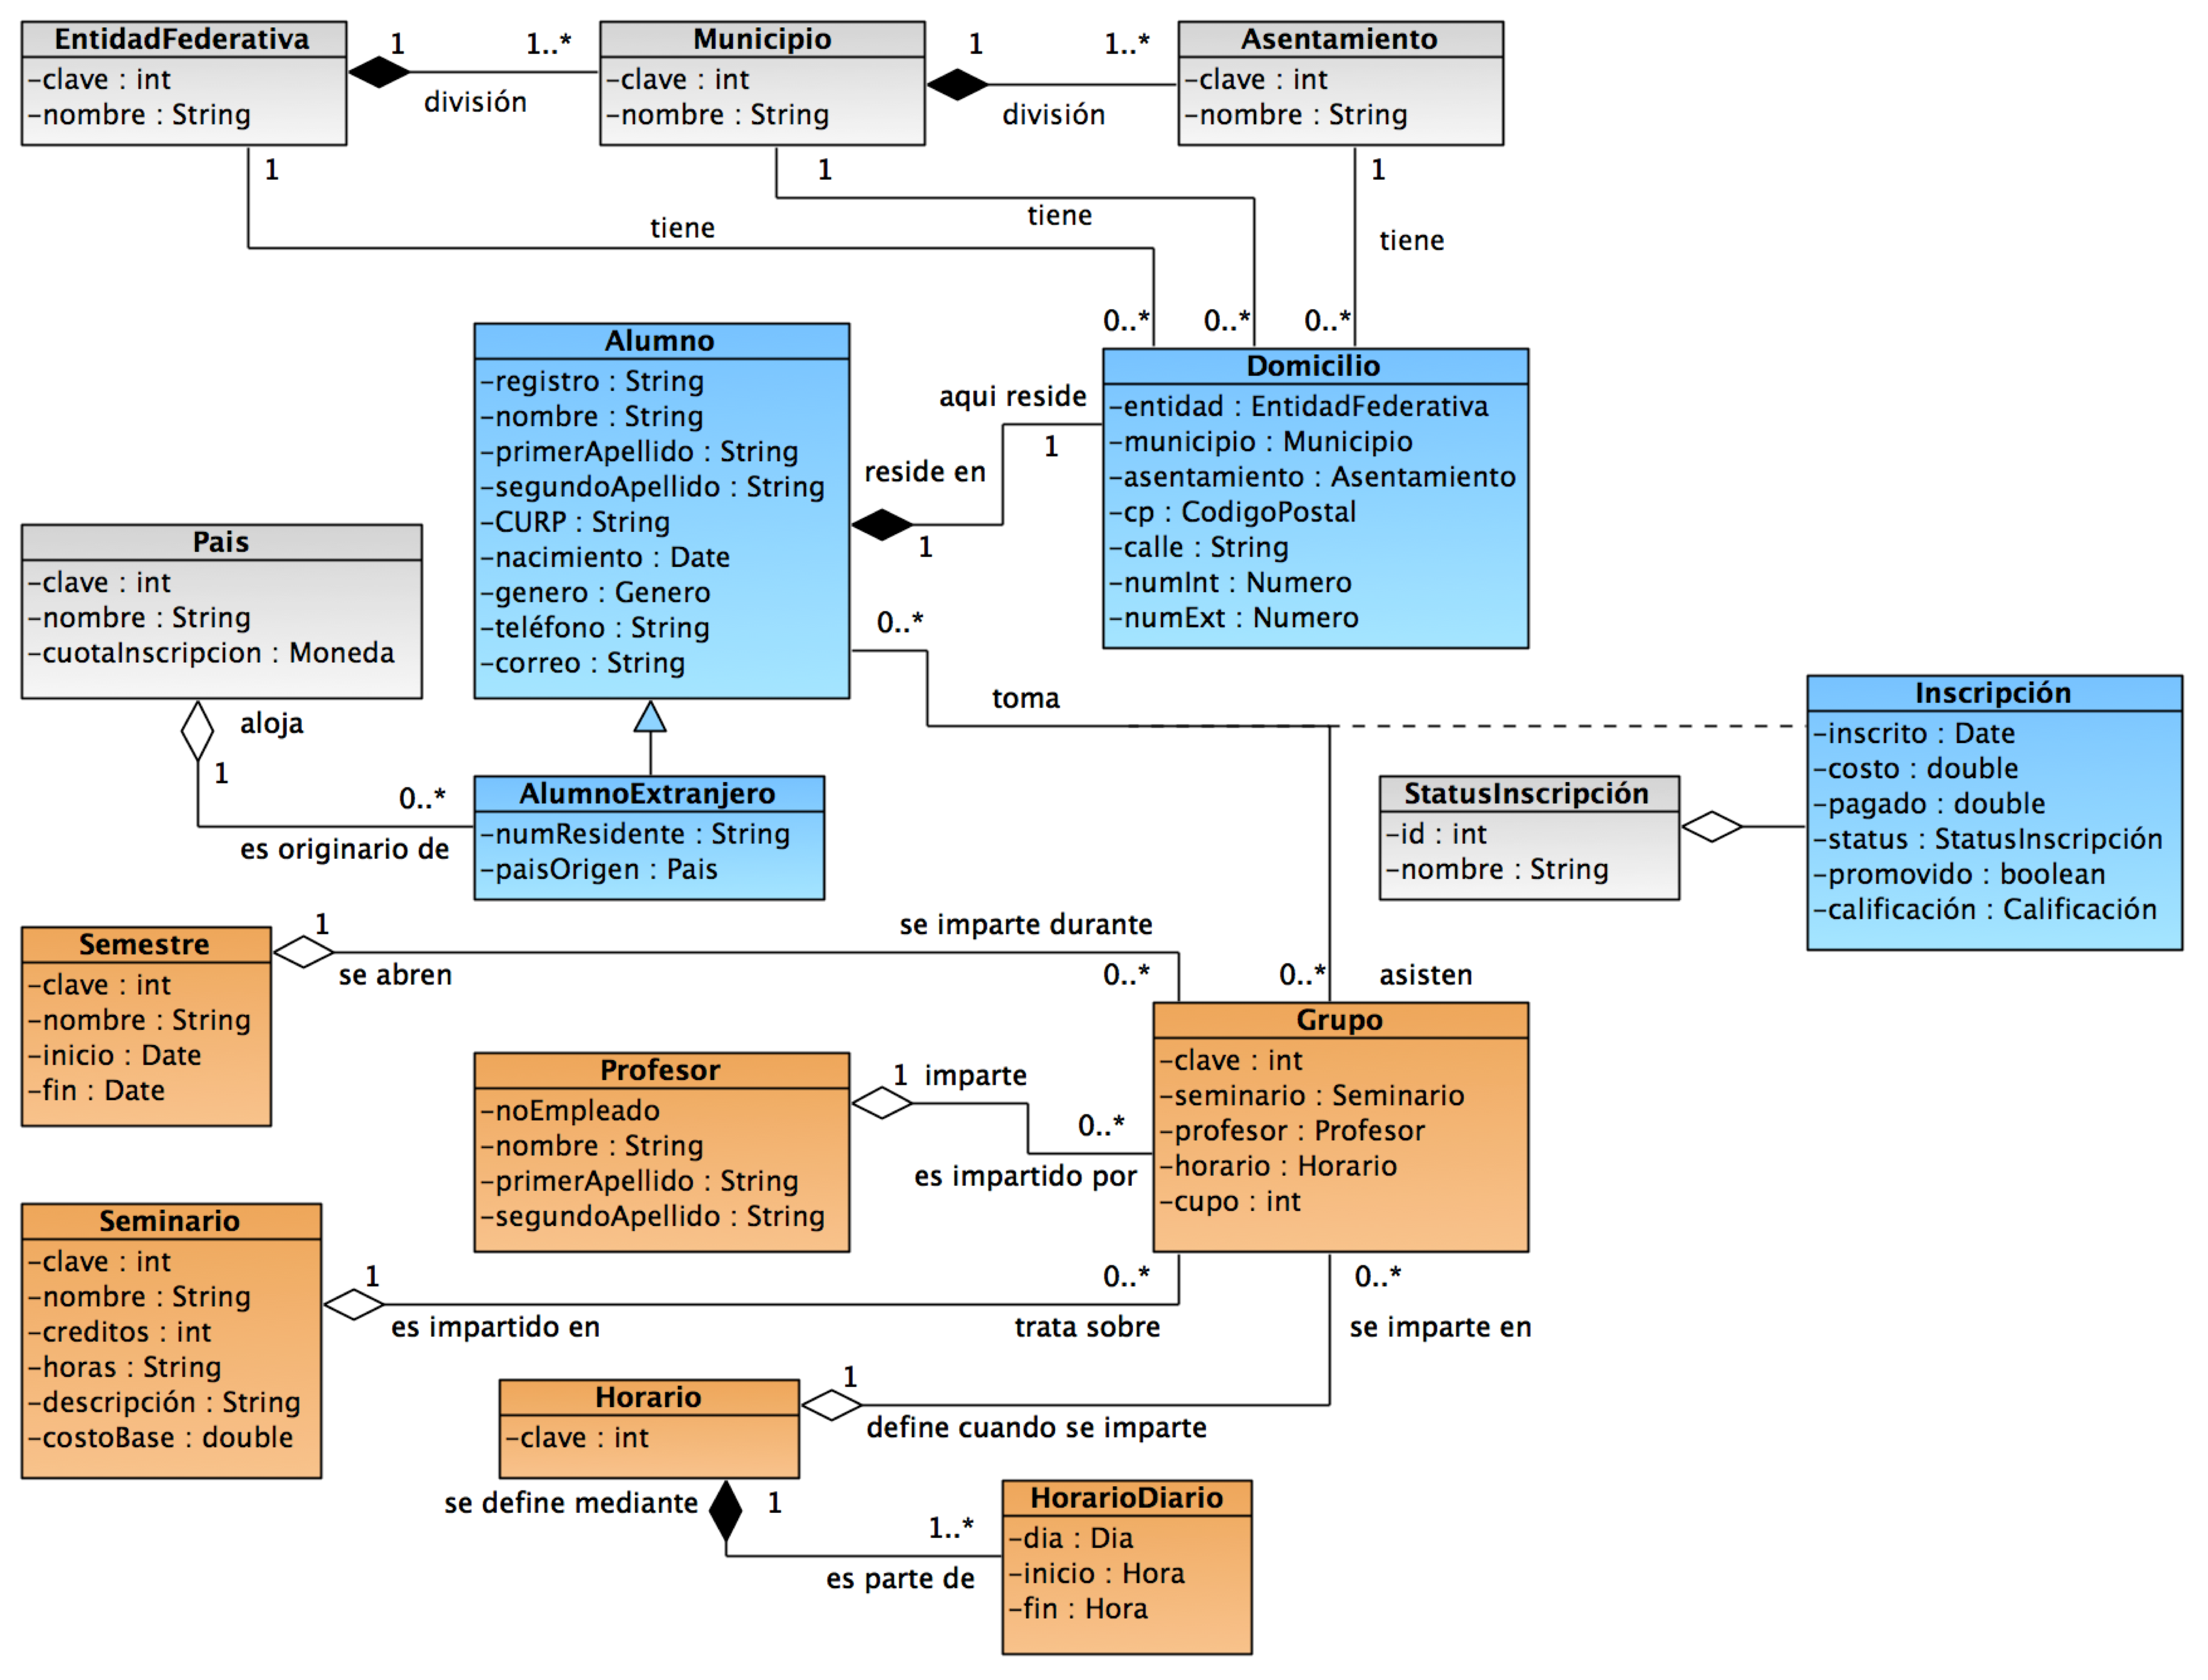
\includegraphics[angle=90,width=.95\textwidth]{images/modeloDelDominioDelProblema}
		\caption{Modelo del dominio del problema}
		\label{fig:modeloDeDominio}
	\end{center}
\end{figure}

\begin{cdtEntidad}{Alumno}{Alumno}
	\brAttr{registro}{Registro}{Id}{Número de registro utilizado para identificar un alumno}{Sí}
	\brAttr{nombre}{Nombre}{Palabra Corta}
		{Nombre o nombres del alumno.}{Sí}
	\brAttr{primerApellido}{Primer apellido}{Palabra Corta}
		{Primer apellido del alumno.}{Sí}
	\brAttr{segundoApellido}{Segundo apellido}{Palabra Corta}
		{Segundo apellido del alumno.}{No}
	\brAttr{CURP}{CURP}{CURP}
		{CURP del alumno.}{Sí}
	\brAttr{nacimiento}{Nacimiento}{Fecha}
		{Fecha de nacimiento del alumno.}{Sí}
	\brAttr{genero}{Género}{Domicilio}
		{Género del alumno.}{No}
	\brAttr{telefono}{Teléfono}{Telefono}
		{Teléfono para contactar al alumno.}{Sí}
	\brAttr{correo}{Correo}{Correo}
		{Correo del alumno para enviar información académica y escolar y para recuperación de clave de acceso.}{Sí}
	\cdtEntityRelSection
	\brRel{\brRelComposition}{Domicilio}{Un \hyperlink{Alumno}{Alumno} reside en un \hyperlink{Domicilio}{Domicilio}}	
	\brRel{\brRelAgregation}{Grupo}{Un \hyperlink{Alumno}{Alumno} toma un \hyperlink{Curso}{Curso}}	
\end{cdtEntidad}

%- - - - - - - - - - - - - - - - - - - - - - - - - - - - - 
\begin{cdtEntidad}{AlumnoExtranjero}{Alumno Extranjero}%{}
	\brAttr{numeroResidente}{Numero de residente}{Id}{Número de registro dado por la Secretaría de Relaciones Exteriores a los extranjeros.}{Si}
	\brAttr{paisOrigen}{Pais origen}{\hyperlink{Pais}{País}}
		{País de origen del alumno extranjero.}{Sí}
	\cdtEntityRelSection
	\brRel{\brRelAgregation}{País}{Un \hyperlink{Alumno}{Alumno} es originario de un \hyperlink{Pais}{Pais}}	
	\brRel{\brRelGeneralization}{Alumno}{Un \hyperlink{AlumnoExtranjero}{Alumno Extranjero} es un  \hyperlink{Alumno}{Alumno}}	
	\brRel{\brRelParticipation}{Alumno}{Un \hyperlink{AlumnoExtranjero}{Alumno Extranjero} es un  \hyperlink{Alumno}{Alumno}}	
\end{cdtEntidad}

%---------------------------------------------------------
\section{Modelado de Reglas de negocio}


% !TeX root = proyecto.tex


\cdtInstrucciones{En esta sección describa todas las reglas de negocio identificadas.}


% Tipo: \btDerivation (no aplica Clase), \btEnabler, \btTimer, \btExecutive
% Clase: \bcCondition, \bcIntegrity, \bcAutorization.
% Cumplimiento: \blStrict \blDeferred \blPreAutorized \blPostJustified \blOverride \blGuideline
\begin{BussinesRule}[%
	\brClassification{\btEnabler}{\bcCondition}{\blStrict}
	]{BR-001}{Nombre de la regla de negocio}
	
				% Opciones para nivel: \blControlling, \blInfluencing
	\BRitem[Descripción:] Descripción de la regla. Forma coloquial a manera de reglamento.
	\BRitem[Motivación:] Describa por que es importante la regla.
	\BRitem[Sentencia:] Sentencia formal de la regla.
	\BRitem[Ejemplo positivo:] Indique uno o varios ejemplos en donde la regla se cumple.
        \begin{itemize}
        	\item ...
        \end{itemize}
	
	\BRitem[Ejemplo negativo:] Indique uno o varios ejemplos en dónde la regla no se cumple.
		\begin{itemize}
        	\item ...
        \end{itemize}
	
	\BRitem[Referenciado por:] Liste los casos de uso en donde la regla no se cumple. por ejemplo \hyperlink{CUCE3.2}{CUCE3.2}, \hyperlink{CUCE3.3}{CUCE3.3}.
\end{BussinesRule}




\section{Máquinas de estado}

% !TeX root = proyecto.tex

\cdtInstrucciones{En esta sección describa para cada máquina de estados y a que entidad corresponde. Utilice reglas ECA en el diagrama y elabore el diagrama de estados, una descripción del diagrama, una descripción de cada estado y una descripción de las acciones indicando que casos de uso están involucrados.}

% - - - - - - - - - - - - - - - - - - - - - - - - - - - - 
\subsection{Estados para un préstamo}

En la figura~\ref{fig:edos-prestamo} se muestran ...

\begin{figure}[htbp]
	\begin{center}
		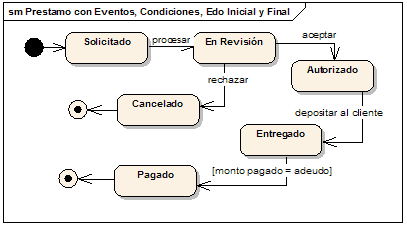
\includegraphics[width=.7\textwidth]{images/edoPrestamo}
		\caption{Máquina de estados de un Préstamo.}
		\label{fig:edos-prestamo}
	\end{center}
\end{figure}

\subsubsection{Estados}

\begin{description}
	\item[Estado:] Descripción del estado.
	\item[...] ...
\end{description}


\subsubsection{Acciones}

\begin{description}
	\item[Acción:] Descripción de la acción indicando el Caso de uso involucrado.
	\item[...] ...
\end{description}




